% -*- latex -*-
%%%%%%%%%%%%%%%%%%%%%%%%%%%%%%%%%%%%%%%%%%%%%%%%%%%%%%%%%%%%%%%%
%%%%%%%%%%%%%%%%%%%%%%%%%%%%%%%%%%%%%%%%%%%%%%%%%%%%%%%%%%%%%%%%
%%%%
%%%% This text file is part of the source of 
%%%% `Parallel Programming in MPI and OpenMP'
%%%% by Victor Eijkhout, copyright 2012-2020
%%%%
%%%% mpi-gatherscatter.tex : about gather & scatter collectives
%%%%
%%%%%%%%%%%%%%%%%%%%%%%%%%%%%%%%%%%%%%%%%%%%%%%%%%%%%%%%%%%%%%%%
%%%%%%%%%%%%%%%%%%%%%%%%%%%%%%%%%%%%%%%%%%%%%%%%%%%%%%%%%%%%%%%%

\Level 0 {Rooted collectives: gather and scatter}
\label{sec:gatherscatter}

\begin{figure}[ht]
  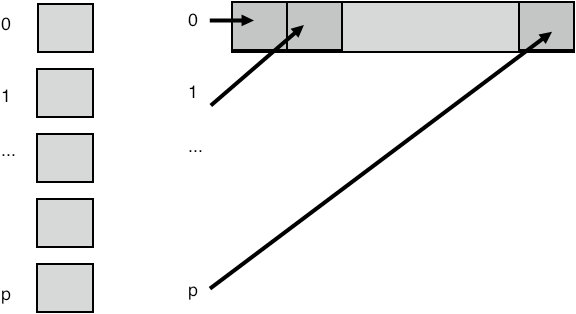
\includegraphics[scale=.4]{gather}
  \caption{Gather collects all data onto a root}
  \label{fig:gather}
\end{figure}

In the \indexmpishow{MPI_Scatter} operation, the root spreads information to
all other processes. The difference with a broadcast is that it involves
individual information from/to every process. Thus, the gather operation typically 
has an array of items, one coming from each sending process, and scatter has an array,
\begin{figure}[ht]
  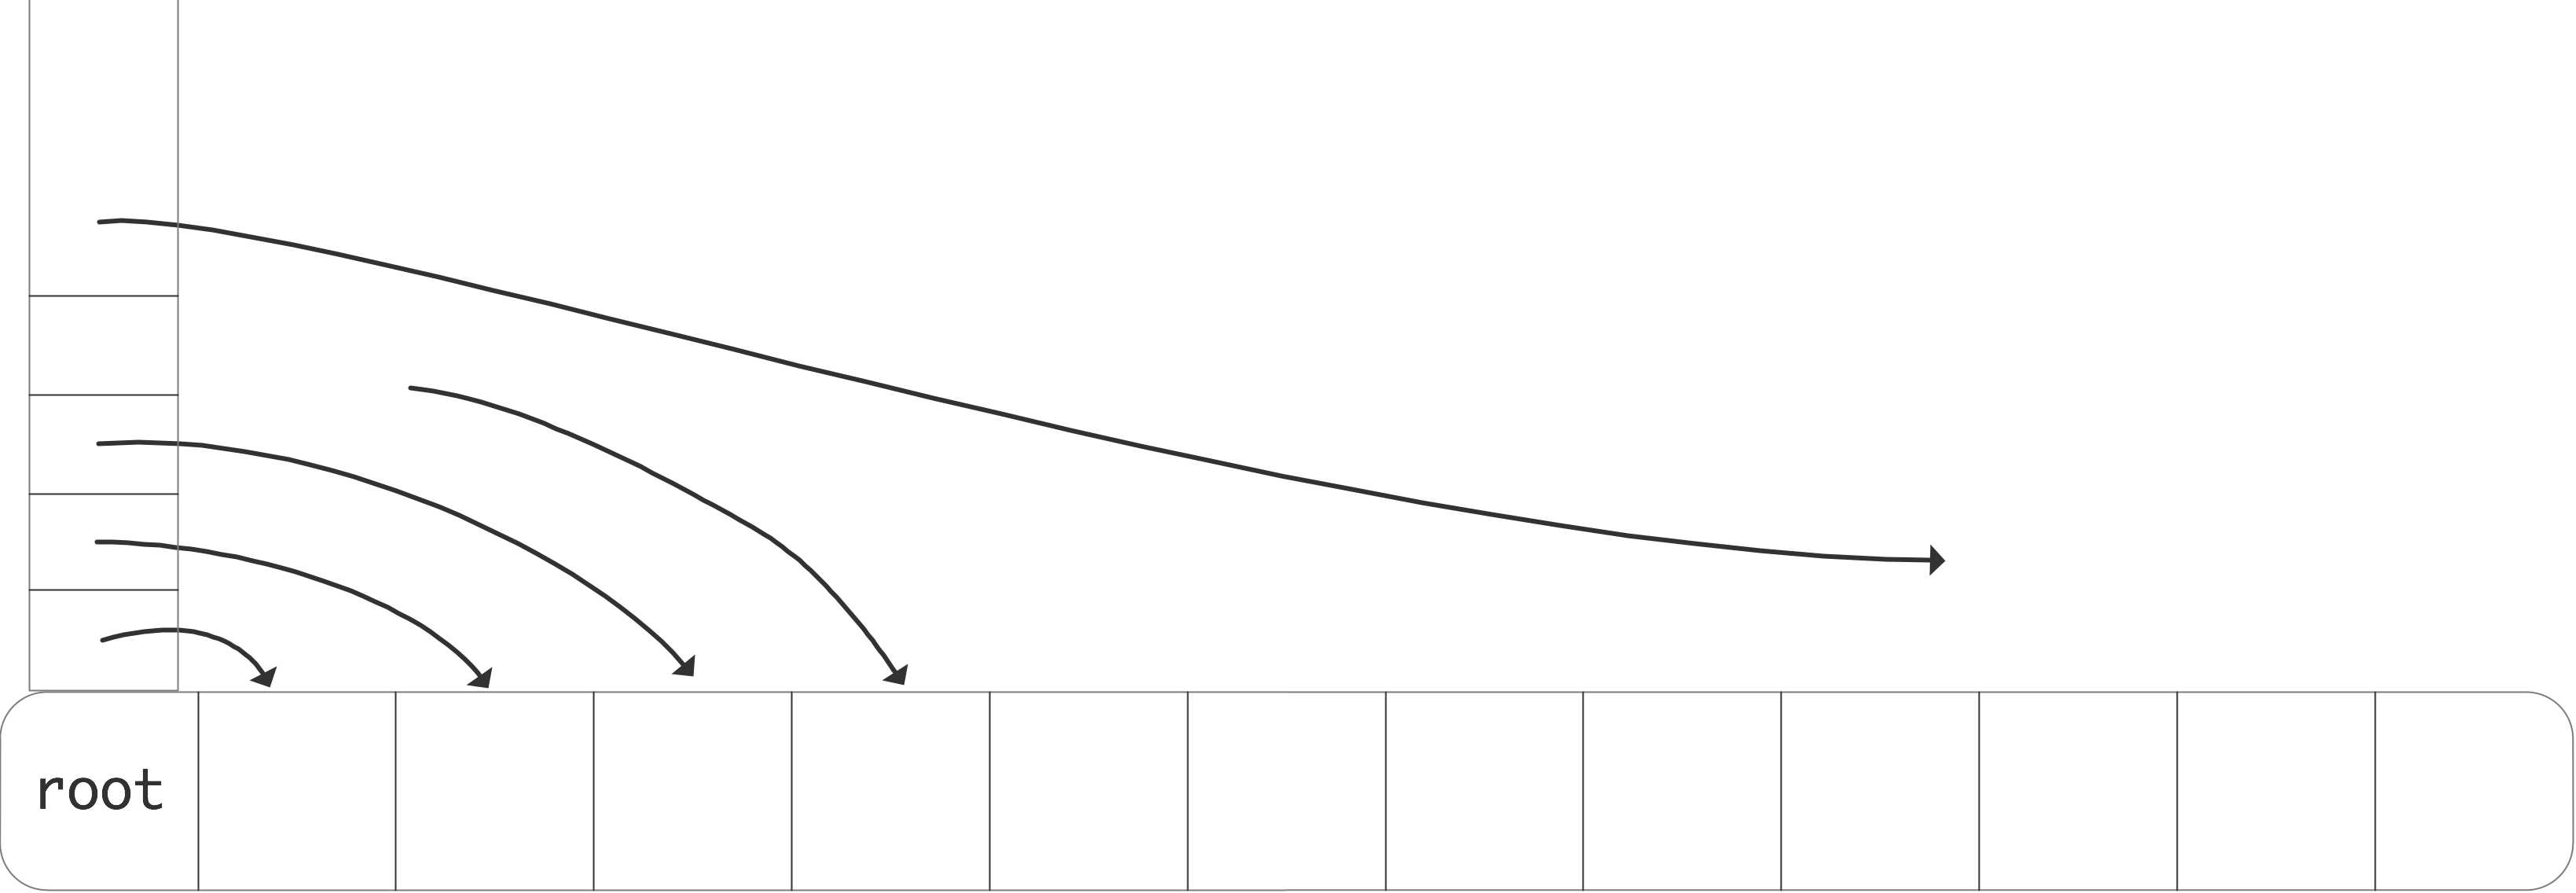
\includegraphics[scale=.12]{graphics/scatter-simple}
  \caption{A scatter operation}
  \label{fig:scatter}
\end{figure}
with an individual item for each receiving process; see figure~\ref{fig:scatter}.

These gather and scatter collectives have a different parameter list from
the broadcast/reduce. The broadcast/reduce involves the same amount
of data on each process, so it was enough to have a single
datatype/size specification; for one buffer in the broadcast, and
for both buffers in the reduce call.
In the gather/scatter calls you have
\begin{itemize}
\item a large buffer on the root, with a datatype and size specification, and
\item a smaller buffer on each process, with its own type and size specification.
\end{itemize}

In the gather and scatter calls, each processor has $n$ elements of individual
data. There is also a root processor that has an array of length~$np$, where $p$
is the number of processors. The gather call collects all this data from the 
processors to the root; the scatter call assumes that the information is 
initially on the root and it is spread to the individual processors.

Here is a small example:
\cverbatimsnippet[examples/mpi/c/gather.c]{gather}
This will also be the basis of a more elaborate example in
section~\ref{sec:v-collective}.

\begin{exercise}
  \label{ex:randomwhere}
  Let each process compute a random number.
  You want to print the maximum value and on what processor it
  is computed. What collective(s) do you use? Write a short program.
\end{exercise}

The \indexmpidef{MPI_Scatter} operation is in some sense the inverse of the gather:
the root process has an array of length $np$ where $p$~is the number of processors
and $n$~the number of elements each processor will receive.
\begin{lstlisting}
int MPI_Scatter
  (void* sendbuf, int sendcount, MPI_Datatype sendtype, 
   void* recvbuf, int recvcount, MPI_Datatype recvtype, 
   int root, MPI_Comm comm) 
\end{lstlisting}

Two things to note about these routines:
\begin{itemize}
\item The prototype for \indexmpiref{MPI_Gather} has two `count' parameters, one
  for the length of the individual send buffers, and one for the receive buffer.
  However, confusingly, the second parameter (which is only relevant on the root)
  does not indicate the total amount of information coming in, but
  rather the size of \emph{each} contribution. Thus, the two count parameters
  will usually be the same (at least on the root); they can differ if you 
  use different \indexmpishow{MPI_Datatype} values for the sending and receiving
  processors.
\item While every process has a sendbuffer in the gather, and a receive buffer
  in the scatter call, only the root process needs the long array in which to gather,
  or from which to scatter.
  However, because in \ac{SPMD} mode all processes need to use the same routine,
  a~parameter for this long array is always present. Non-root processes can use
  a \indextermsub{null}{pointer} here.
\item More elegantly, the \indexmpishow{MPI_IN_PLACE} option can be
  used buffers that are not applicable. See section~\ref{sec:allreduce-inplace}.
\end{itemize}

\begin{mplnote}{Gather/scatter}
  Gathering (by \indexmpldef{gather}) or scattering (by \indexmpldef{scatter})
  a single scalar takes a scalar argument
  and a raw array:
  %
  \cxxverbatimsnippet[examples/mpi/mpl/collectbuffer.cxx]{mplscattergatherx}
  %
  If more than a single scalar is gathered, or scattered into,
  it becomes necessary to specify a layout:
  %
  \cxxverbatimsnippet[examples/mpi/mpl/collectbuffer.cxx]{mplscattergatherv}  
\end{mplnote}

\Level 1 {Examples}

In some applications, each process computes a row or column of a
matrix, but for some calculation (such as the determinant) it is more
efficient to have the whole matrix on one process. You should of
course only do this if this matrix is essentially smaller than the
full problem, such as an interface system or the last coarsening level
in multigrid.

\begin{figure}[ht]
  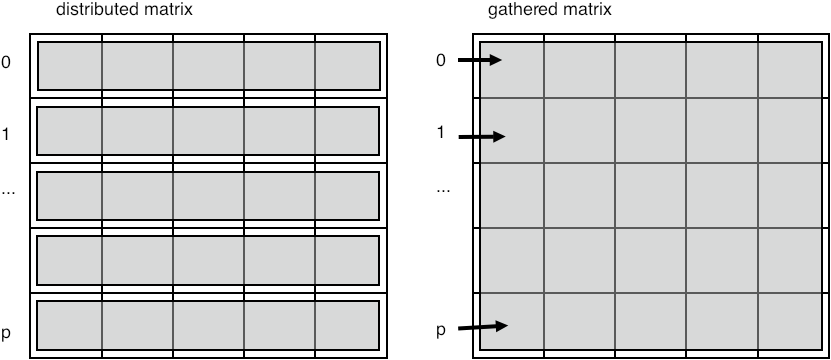
\includegraphics[scale=.4]{allgathermatrix}
  \caption{Gather a distributed matrix onto one process}
  \label{fig:allgathermatrix}
\end{figure}

Figure~\ref{fig:allgathermatrix} pictures this. Note that conceptually
we are gathering a two-dimensional object, but the buffer is of course
one-dimensional. You will later see how this can be done more
elegantly with the `subarray' datatype; section~\ref{sec:type_subarray}.

Another thing you can do with a distributed matrix is to transpose it.
%
\cverbatimsnippet[examples/mpi/c/itransposeblock.c]{transposescatterref}
%
In this example, each process scatters its column.
This needs to be done only once, yet the scatter happens in a loop.
The trick here is that a process only originates the scatter when it
is the root, which happens only once.
Why do we need a loop? That is because each element of a process' row
originates from a different scatter operation.

\begin{exercise}
  Can you rewrite this code so that it uses a gather rather than a scatter?
  Does that change anything essential about structure of the code?
\end{exercise}

\Level 1 {Allgather}

\begin{figure}[ht]
  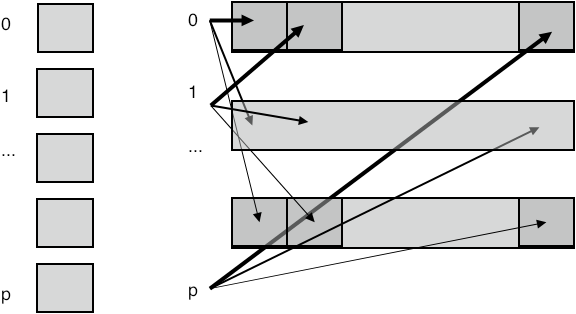
\includegraphics[scale=.4]{allgather}
  \caption{All gather collects all data onto every process}
  \label{fig:allgather}
\end{figure}

The \indexmpiref{MPI_Allgather} routine does the same gather onto
every process: each process winds up with the totality of all data;
figure~\ref{fig:allgather}.

This routine can be used in the simplest implementation of the 
%
\indextermsub{dense}{matrix-vector product} to give each processor the
full input; see~\HPSCref{sec:densescaling}.

Some cases look like an all-gather but can be implemented more
efficiently. Suppose you have two distributed vectors, and you want to
create a new vector that contains those elements of the one that do
not appear in the other. You could implement this by gathering the
second vector on each processor, but this may be prohibitive in memory
usage.

\begin{exercise}
  Can you think of another algorithm for taking the set difference of
  two distributed vectors. Hint: look up `bucket-brigade algorithm'
  in~\cite{Eijkhout:IHPSClulu}. What is the time and space complexity
  of this algorithm? Can you think of other advantages beside a
  reduction in workspace?
\end{exercise}
